%% LyX 2.1.4 created this file.  For more info, see http://www.lyx.org/.
%% Do not edit unless you really know what you are doing.
\RequirePackage{fix-cm}
\documentclass[english,envcountsect]{beamer}
\usepackage[latin9]{inputenc}
\setcounter{secnumdepth}{3}
\setcounter{tocdepth}{3}
\usepackage{array}
\usepackage{amsmath}
\usepackage{amsthm}
\usepackage{amssymb}

\makeatletter

%%%%%%%%%%%%%%%%%%%%%%%%%%%%%% LyX specific LaTeX commands.
\special{papersize=\the\paperwidth,\the\paperheight}

%% Because html converters don't know tabularnewline
\providecommand{\tabularnewline}{\\}

%%%%%%%%%%%%%%%%%%%%%%%%%%%%%% Textclass specific LaTeX commands.
 % this default might be overridden by plain title style
 \newcommand\makebeamertitle{\frame{\maketitle}}%
 % (ERT) argument for the TOC
 \AtBeginDocument{%
   \let\origtableofcontents=\tableofcontents
   \def\tableofcontents{\@ifnextchar[{\origtableofcontents}{\gobbletableofcontents}}
   \def\gobbletableofcontents#1{\origtableofcontents}
 }
  \newenvironment{sol}{\begin{proof}[Solution.]\renewcommand{\qedsymbol}{}}{\end{proof}}

%%%%%%%%%%%%%%%%%%%%%%%%%%%%%% User specified LaTeX commands.
\usepackage{tikz}
\usepackage{pgf}
\usepackage{graphicx}
%\usepackage{mathabx}
%\newref{prop}{refcmd = {proposition \ref{#1}}}
%\newref{le}{refcmd = {lemma \ref{#1}}}
%\newref{def}{refcmd = {definition \ref{#1}}}
\usetheme{Berkeley}
\usecolortheme{wolverine}
\setbeamertemplate{section in toc}{\hspace*{1em}{\color{structure}\rule[0.5ex]{4pt}{4pt}}~\inserttocsection}
\setbeamertemplate{subsection in toc}{\hspace*{2em}{\color{structure}\rule[0.5ex]{4pt}{4pt}}~\inserttocsubsection\par}

\setbeamercovered{transparent}
% or whatever (possibly just delete it)
\setbeamertemplate{theorems}[numbered]
%\includeonlylecture{test2}
\AtBeginSection{
\begin{frame}{\insertsection}
\origtableofcontents[currentsection]
\end{frame}}

\makeatother

\usepackage{babel}
\begin{document}
\tikzset{
    invisible/.style={opacity=0},
    visible on/.style={alt={#1{}{invisible}}},
    alt/.code args={<#1>#2#3}{%
      \alt<#1>{\pgfkeysalso{#2}}{\pgfkeysalso{#3}} % \pgfkeysalso doesn't change the path
    },
  }
%This for step by step unvealing objects in tikz picture.
%You only need to add "visible on = <1->" in the options of that object. Notice that if you want something to show on the page 1,3, you need use <{1,3}>


\title{AP Review\thanks{All the page numbers are refered to the calculus textbook by Anton
Bivens and Davis.}}


\author[Y. Sun]{Yitong Sun}


\institute[UofM]{University of Michigan}

\makebeamertitle

%\section{Functions}
\begin{frame}{Inverse function}

\begin{onlyenv}<1>

\begin{itemize}
\item A function and its inverse function reflect the same relation from
different direction. When you buy coffee in a Starbucks, you will
deal with the following function $c=f\left(n\right)$.


\begin{center}
\begin{tabular}{|c|c|c|c|c|}
\hline 
$n$ & 1 & 2 & 3 & 4\tabularnewline
\hline 
$c$ $\left(\$\right)$ & 6 & 12 & 17 & 20\tabularnewline
\hline 
\end{tabular}
\par\end{center}


Its inverse $n=f^{-1}\left(c\right)$ is just to read the table from
second row to the first row.

\item Do not switch the letters for variables, especially in a real problem.
\item \alert{Horizontal line test} helps you determine whether the function
has an inverse or not.
\end{itemize}
\end{onlyenv}



\begin{onlyenv}<2>

\begin{itemize}
\item The domain of $f$ is the range of $f^{-1}$ and the range of $f$
is the domain of $f^{-1}$.
\item $f\circ f^{-1}\left(x\right)=x$ and $f^{-1}\circ f\left(x\right)=x$.
For example,
\[
\ln\left(e^{x}\right)=e^{\ln x}=x
\]

\end{itemize}
\end{onlyenv}



\begin{onlyenv}<3>

\begin{example}
p49-7
\end{example}

\end{onlyenv}

\end{frame}

\begin{frame}{Polynomials}

\begin{itemize}
\item $f\left(x\right)=a_{n}x^{n}+a_{n-1}x^{n-1}+\cdots+c_{1}x+c_{0}$
\item The long term behavior of a polynomial is determined by its \alert{leading term}.
This is very useful in evaluating \alert{limits}.
\item How to solve $\left(x-1\right)\left(x^{2}-2\right)<0$?
\end{itemize}
\end{frame}

\begin{frame}{Rational functions}

\begin{itemize}
\item $f\left(x\right)=\frac{P\left(x\right)}{Q\left(x\right)}$, where
$P$ and $Q$ are two polynomials.
\item How to find out the asymptotes of
\[
y=\frac{2x^{2}-x}{3x^{2}+2x-1}
\]

\item How to solve
\[
\frac{x-2}{x+1}<2x
\]

\end{itemize}
\end{frame}

\begin{frame}{Trig and anti-trig}

\begin{itemize}
\item Draw the graph of $\sin$, $\cos$, $\tan$.
\item State the the domain and range of $\arcsin/\sin^{-1}$, $\arccos/\cos^{-1}$,
$\arctan/\tan^{-1}$.\end{itemize}
\begin{example}
p50-46, p64-22
\end{example}

\end{frame}

\begin{frame}{Exp and log functions}

\begin{onlyenv}<1>

\begin{itemize}
\item Sketch the graph of $y=e^{x}$, $y=e^{-x}$, $y=\ln x$.
\item Laws of exponents:
\[
a^{0}=\quad,a^{1}=\quad,a^{m}\cdot a^{n}=\quad,a^{m}/a^{n}=\quad,
\]
\[
\left(a^{m}\right)^{n}=\quad,a^{-m}=\quad.
\]

\item Laws of log:
\[
\log_{a}1=\quad,\log_{a}a=\quad,
\]
\[
\log_{a}mn=
\]
\[
\log_{a}\frac{m}{n}=
\]
\[
\log_{a}x^{m}=
\]

\end{itemize}
\end{onlyenv}



\begin{onlyenv}<2>

\begin{example}
p61-28, p62-50, p65-38
\end{example}

\end{onlyenv}

\end{frame}

\begin{frame}{Parametric curve}

\begin{onlyenv}<1>


\[
\begin{cases}
x=f\left(t\right)\\
y=g\left(t\right)
\end{cases}
\]
gives a curve as the trace of the particle $P\left(x,y\right)$.

\end{onlyenv}



\begin{onlyenv}<2>

\begin{example}
Sketch the graph given by
\[
x=1-t,\quad y=\sqrt{t}\mbox{ for }t\ge0
\]
without using graphing calculator.
\end{example}



\begin{example}
Sketch the graph given by
\[
x=4\cos t+\cos12t,\quad y=4\sin t+\sin12t\mbox{ for }0\le t\le2\pi
\]
using graphing calculator.
\end{example}

\end{onlyenv}

\end{frame}

\begin{frame}{Polar coordinates}

\begin{itemize}
\item Sketch the following curves in polar coordinates plane
\[
r=\theta
\]
\[
r=1+3\cos\theta
\]

\end{itemize}
\end{frame}

%\section[Limits]{Limits and Continuity}
\begin{frame}{Basic limits}


\[
\lim_{x\to\infty}\frac{1}{x}=\quad,\lim_{x\to0-}\frac{1}{x}=\quad,\lim_{x\to0}\frac{\sin x}{x}=\quad
\]
\[
\lim_{x\to0+}\left(1+x\right)^{1/x}=\quad,\lim_{x\to\infty}\arctan x=\quad\lim_{x\to\infty}e^{-x}=
\]

\begin{example}
p128-4
\end{example}

\end{frame}

\begin{frame}{Limits laws}


\[
\lim_{x\to0+}\left[\left(1+x\right)^{1/x}+\frac{\sin x}{x}\right]=
\]
\[
\lim_{x\to\infty}\left(\frac{2}{x}-\frac{1}{x^{2}}\right)=
\]
\[
\lim_{x\to0}\frac{x}{x}=
\]


\end{frame}

\begin{frame}{Limits of continuous functions}

\begin{onlyenv}<1>


If $f$ is continuous,
\[
\lim_{x\to2}f\left(x\right)=
\]
\[
\lim_{x\to\infty}f\left(\frac{1}{x}\right)=
\]


\end{onlyenv}



\begin{onlyenv}<2>

\begin{example}
p128-1(a),(h),
\[
\lim_{x\to\infty}f\left(\frac{3x}{x-1}\right)\,,\lim_{x\to0}f\left(\frac{3x}{x}\right)\,.
\]

\end{example}

\end{onlyenv}

\end{frame}

\begin{frame}{Squeeze theorem}


For $f\left(x\right)=x^{2}\sin x$, $-x^{2}\le f\left(x\right)\le x^{2}$,
because
\[
\lim_{x\to0}-x^{2}=\lim_{x\to0}x^{2}=0
\]
So
\[
\lim_{x\to0}x^{2}\sin x=0\,.
\]


\end{frame}

\begin{frame}{More techniques}

\begin{onlyenv}<1>

\begin{itemize}
\item For rational functions $\frac{P\left(x\right)}{Q\left(x\right)}$

\begin{enumerate}
\item Find out the highest leading term among $P\left(x\right)$ and $Q\left(x\right)$;
\item Divide $P\left(x\right)$ and $Q\left(x\right)$ by the leading term;
\item Evaluate the limit.
\end{enumerate}
\end{itemize}
\begin{example}
\[
\lim_{x\to\infty}\frac{3-x}{4+x+x^{2}}
\]
\[
\lim_{x\to-\infty}\frac{4+x^{2}-3x^{3}}{x+7x^{3}}
\]



\end{example}

\end{onlyenv}



\begin{onlyenv}<2>

\begin{itemize}
\item For $\frac{\sin mx}{nx}$

\begin{enumerate}
\item Transform
\[
\frac{\sin mx}{nx}\longrightarrow\frac{\sin mx}{mx}\cdot\frac{mx}{nx}\,;
\]

\item Use the fact to evaluate
\[
\frac{\sin mx}{mx}\,;
\]

\item Use limit laws to obtain final result.
\end{enumerate}
\end{itemize}
\end{onlyenv}



\begin{onlyenv}<3>

\begin{itemize}
\item $\left(1+mx\right)^{1/nx}$ related

\begin{enumerate}
\item Find appropriate transformation so that ``$\square$'' represent
the same thing in the expression $\left(1+\square\right)^{1/\square}$.
For example,
\[
\left(1+mx\right)^{1/nx}\longrightarrow\left[\left(1+mx\right)^{1/mx}\right]^{m/n}
\]

\item Then use the fact
\[
\lim_{\square\to0}\left(1+\square\right)^{1/\square}=e\,.
\]

\end{enumerate}
\end{itemize}
\end{onlyenv}



\begin{onlyenv}<4>

\begin{itemize}
\item Recognized as a derivative
\item l'Hospital's rule
\end{itemize}
\end{onlyenv}

\end{frame}

\begin{frame}{Continuity}

\begin{onlyenv}<1>

\begin{itemize}
\item Definition
\[
\lim_{x\to a-}f\left(x\right)=\lim_{x\to a+}f\left(x\right)=f\left(a\right)
\]

\item Terms: removable, jump, infinity discontinuity
\item Properties: Extreme value theorem, Intermediate value theorem
\item \alert{All the elementary functions and their combination and composition
are continuous in their domain!}
\item Be careful about such expression
\[
\frac{x^{2}-1}{x+1}\,.
\]

\end{itemize}
\end{onlyenv}



\begin{onlyenv}<2>

\begin{example}
p118-5, 6
\end{example}

\end{onlyenv}

\end{frame}




%\section{Differentiation}
\begin{frame}{Definition of derivative}


Derivative is defined as the limit of difference quotient,
\[
\frac{\mathrm{d}}{\mathrm{d}x}f\left(x\right)=f'\left(x\right)=\lim_{\Delta x\to0}\frac{f\left(x+\Delta x\right)-f\left(x\right)}{\Delta x}\,.
\]

\begin{onlyenv}<2-4>

\begin{itemize}
\item The difference quotient is the slope of \uncover<3-4>{secant line}.
\item Its limit, the derivative, is the slope of \uncover<4>{tangent line}.
\end{itemize}
\end{onlyenv}



\begin{onlyenv}<5-7>

\begin{itemize}
\item The difference quotient is the \uncover<6-7>{average} rate of change.
\item Its limit, the derivative, is the \uncover<7>{instantaneous} rate
of change.
\end{itemize}
\end{onlyenv}

\end{frame}

\begin{frame}{Derivatives of basic functions}

\begin{onlyenv}<1>


Derivative of $\tan(x)$, $a^{x}$, $\arcsin(x)$, $\arccos(x)$,
$\arctan(x)$.

\end{onlyenv}



\begin{onlyenv}<2>

\begin{example}
If $y=\left(x^{2}+x\right)\cdot\sin x$, find $y'\left(\frac{\pi}{2}\right)$
and $y''\left(\frac{\pi}{2}\right)$.
\end{example}



\begin{example}
If $f\left(v\right)=\frac{2v}{1-2v^{2}}$, find $f'\left(v\right)$.
\end{example}

\end{onlyenv}

\end{frame}

\begin{frame}{Chain rule}

\begin{example}
If $f\left(x\right)=\left(3x+2\right)^{5}$, then find $f'\left(x\right)$.
\end{example}



\begin{example}
If $f\left(x\right)=\frac{5}{\sqrt{\left(1-x^{2}\right)^{3}}}$, find
$f'\left(x\right)$.
\end{example}



\begin{example}
p181-75
\end{example}

\end{frame}

\begin{frame}{Differentiability and continuity}


Differentiability implies continuity,


but continuity does not imply differentiability.


Think about the graph of $\left|x\right|$ and $x^{1/3}$.


\pause{}
\begin{example}
p182-10
\end{example}

\end{frame}

\begin{frame}{Estimating a derivative}

\begin{example}
Numerically, p153-39,40
\end{example}


\pause{}
\begin{example}
Graphically, p142-24, p180-68
\end{example}

\end{frame}

\begin{frame}{Derivatives of parametric curves}

\begin{onlyenv}<1>


\[
\frac{\mathrm{dy}}{\mathrm{d}x}=\frac{\frac{\mathrm{d}y}{\mathrm{d}t}}{\frac{\mathrm{d}x}{\mathrm{d}t}}
\]
\[
\frac{\mathrm{d}^{2}y}{\mathrm{d}x^{2}}=\frac{\frac{\mathrm{d}}{\mathrm{d}t}\left(\frac{\mathrm{d}y}{\mathrm{d}x}\right)}{\frac{\mathrm{d}x}{\mathrm{d}t}}
\]


\end{onlyenv}



\begin{onlyenv}<2>

\begin{example}
Find the equation of the tangent to the curve given by
\[
\begin{cases}
x=2\sin\theta\\
y=\cos2\theta
\end{cases}
\]
for $\theta=\frac{\pi}{6}$.


\end{example}

\end{onlyenv}

\end{frame}

\begin{frame}{Implicit differentiation}


\alert{Just remember, every thing in the equation is a function of independent
variable. That means you need apply Product, Quotient and Chain rule
to them.}
\begin{example}
Find the derivative $y'$ and $y''$ for
\[
x^{2}-2xy+3y^{2}=2
\]
and
\[
x\sin y=\cos\left(x+y\right)
\]



\end{example}

\end{frame}

\begin{frame}{Derivative of the inverse of a function}

\begin{onlyenv}<1>


If a function $y=f\left(x\right)$ has its inverse $x=f^{-1}\left(y\right)$.
Then
\begin{eqnarray*}
f^{-1}\left(f\left(x\right)\right) & = & x\\
\frac{\mathrm{d}}{\mathrm{d}y}f^{-1}\left(y\right)\bigg|_{y=f\left(x\right)}\cdot\frac{\mathrm{d}}{\mathrm{d}x}f\left(x\right) & = & 1\\
\frac{\mathrm{d}}{\mathrm{d}y}f^{-1}\left(y\right)\bigg|_{y=f\left(x\right)} & = & \frac{1}{\frac{\mathrm{d}}{\mathrm{d}x}f\left(x\right)}\,.
\end{eqnarray*}


\end{onlyenv}



\begin{onlyenv}<2,3>

\begin{example}
If $f\left(3\right)=8$ and $f'\left(3\right)=5$, what do we know
about $f^{-1}$?\end{example}

\begin{uncoverenv}<3>

\begin{sol}
First, $f^{-1}\left(8\right)=3$.

\[
\frac{\mathrm{d}}{\mathrm{d}y}f^{-1}\bigg|_{y=8}=\frac{1}{\frac{\mathrm{d}}{\mathrm{d}x}f\bigg|_{x=3}}=\frac{1}{5}\,.
\]

\end{sol}
\end{uncoverenv}

\end{onlyenv}



\begin{onlyenv}<4>

\begin{example}
Let $y=f\left(x\right)=x^{3}+x-2$, and let $g$ be the inverse function.
Evaluate $g'\left(0\right)$.
\end{example}

\end{onlyenv}

\end{frame}

\begin{frame}{The mean value theorem (differentiation)}

\begin{onlyenv}<1>


\[
\frac{f\left(b\right)-f\left(a\right)}{b-a}=f'\left(c\right)\mbox{ for some }c\in\left(a,b\right)\,.
\]
Verbally, the \alert{average rate of change} of some function $f$
on some interval 


equals the \alert{instantaneous rate of change} at some point in
that interval.

\end{onlyenv}



\begin{onlyenv}<2>

\begin{example}
You left home one morning and drove to a cousin's house $300$ miles
away, arriving $6$ hours later. What does the mean value theorem
say about your speed along the way?
\end{example}

\end{onlyenv}

\end{frame}

\begin{frame}{l'Hôspital's rule}

\begin{onlyenv}<1>

\begin{enumerate}
\item First, the expression must be an indeterminate form.
\item Find derivatives of the denominator and numerator.
\item Compute the limit of quotient of derivatives.

\begin{enumerate}
\item If the limit exists or equals $\infty$, then it is the value of the
original limit;
\item if the limit does not exist, then we cannot get a conclusion;
\item if the it is still an indeterminate form, repeat step 2.
\end{enumerate}
\end{enumerate}
\end{onlyenv}



\begin{onlyenv}<2>

\begin{example}
$\lim_{x\to-2}\frac{x^{3}+8}{x^{2}-4}$
\end{example}



\begin{example}
$\lim_{x\to2}\frac{x^{3}+8}{x^{2}+4}$
\end{example}



\begin{example}
$\lim_{x\to\infty}x\sin\frac{1}{x}$
\end{example}

\end{onlyenv}

\end{frame}

\begin{frame}{Recognize a given limit as a derivative}

\begin{example}
$\lim_{h\to0}\frac{\left(2+h\right)^{4}-2^{4}}{h}$
\end{example}



\begin{example}
$\lim_{h\to0}\frac{1}{h}\left(\frac{1}{2+h}-\frac{1}{2}\right)$
\end{example}

\end{frame}




%\section[AppofDiff]{Application of Differential Calculus}
\begin{frame}{Slope of tangent lines}

\begin{onlyenv}<+>

\begin{example}
Find the equations of the tangent and normal to the curve of $f\left(x\right)=x^{3}-3x^{2}$
at the point $\left(1,-2\right)$.
\end{example}



\begin{example}
Find the equation of the tangent to $x^{2}y-x=y^{3}-8$ at the point
where $x=0$.
\end{example}

\end{onlyenv}



\begin{onlyenv}<+>

\begin{example}
Find the coordinates of any point on the curve of $y^{2}-4xy=x^{2}+5$
for which the tangent is horizontal.
\end{example}



\begin{example}
(slope of parametric curves) Find the equation of the tangent to $F\left(t\right)=\left(\cos t,2\sin^{2}t\right)$
at the point where $t=\frac{\pi}{3}$.
\end{example}



\begin{example}
(slope of polar curves) Find the slope of the cardioid $r=2\left(1+\cos\theta\right)$
at $\theta=\frac{\pi}{6}$. Where is the tangent to the curve horizontal?
\end{example}

\end{onlyenv}

\end{frame}

\begin{frame}{Average and instantaneous rates of change}

\begin{onlyenv}<1>

\begin{itemize}
\item Average rate of change
\[
\frac{f\left(a+h\right)-f\left(a\right)}{h}\,,\quad\frac{f\left(b\right)-f\left(a\right)}{b-a}\,.
\]

\item Instantaneous rate of change/derivative
\[
\lim_{h\to0}\frac{f\left(a+h\right)-f\left(a\right)}{h}\,,\quad\lim_{b\to a}\frac{f\left(b\right)-f\left(a\right)}{b-a}\,.
\]

\end{itemize}
\end{onlyenv}



\begin{onlyenv}<2>

\begin{example}
Let $G\left(t\right)=400\left(15-t\right)^{2}$ be the number of gallons
of water in a tank $t$ minutes after an outlet pipe is opened. Find
the average rate of drainage during the first $5$ minutes and the
rate at which the water is running out at the end of $5$ minutes.
\end{example}

\end{onlyenv}

\end{frame}

\begin{frame}{Monotonicity, concavity and local extrema}

\begin{onlyenv}<1>


\begin{center}
\begin{tabular}{|>{\raggedleft}p{0.15\columnwidth}|>{\raggedright}p{0.23\columnwidth}|>{\raggedright}p{0.23\columnwidth}|>{\raggedright}p{0.23\columnwidth}|}
\hline 
 & {\small{}$f$} & {\small{}$f'$} & {\small{}$f''$}\tabularnewline
{\small{}$>0$} & {\small{}positive} & {\small{}increasing} & {\small{}concave up}\tabularnewline
{\small{}$<0$} & {\small{}negative} & {\small{}decreasing} & {\small{}concave down}\tabularnewline
{\small{}$=0$} & {\small{}roots} & {\small{}possible local extremes} & {\small{}possible inflection point}\tabularnewline
{\small{}not exist} & {\small{}out of domain} & {\small{}possible local extremes} & {\small{}possible inflection point}\tabularnewline
\hline 
\end{tabular}
\par\end{center}
\begin{itemize}
\item For the possible extremes/inflection points, you need to check the
trend around that point. Always remember the examples of $x^{3}$
and $x^{4}$.
\item The points at which $f'$ equals $0$ or does not exist are called
\alert{critical points}.
\end{itemize}
\end{onlyenv}



\begin{onlyenv}<2,3>

\begin{example}
Find all the local maximum, minimum, inflection points on the graph
of $f\left(x\right)=x^{3}-5x^{2}+3x+6$ and sketch the graph.
\end{example}
\uncover<3>{
\begin{example}
p241-3, 4, 5; p242-11 to 14, 40, 46; p252-18
\end{example}
}
\end{onlyenv}

\end{frame}

\begin{frame}{Global minimum or maximum}

Based on the analysis of local/relative extremum, take the values
at end points into account.
\begin{example}
p272-17 to 20; p273-43, 44
\end{example}

\end{frame}

\begin{frame}{Optimization}

\begin{onlyenv}<1-6>
\begin{enumerate}[<+->]
\item Find out the \alt<+->{dependent variable}{quantity we want to optimize};
\item Find out the \alt<+->{independent variables}{factor that changes the quantity we study};
\item Establish a function between dependent and independent variables;
\item Find out the (usually global) maximum/minimum. Remember to use the correct domain.
\end{enumerate}
\end{onlyenv}

\begin{onlyenv}<+>

\begin{example}
The region in the first quadrant bounded by the curves of $y^{2}=x$
and $y=x$ is rotated about the $y$-axis to form a solid. Find the
area of the largest cross section of this solid that is perpendicular
to the $y$-axis.

\begin{center}
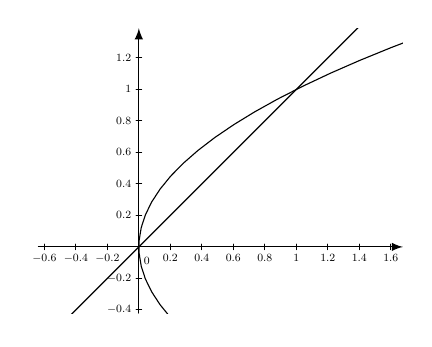
\begin{tikzpicture}[line cap=round,line join=round,>=latex,x=4.0cm,y=4.0cm,scale=0.5,transform shape]
\draw[->,color=black] (-0.6382410397208873,0.) -- (1.6766681092950013,0.);
\foreach \x in {-0.6,-0.4,-0.2,0.2,0.4,0.6,0.8,1,1.2,1.4,1.6}
\draw[shift={(\x,0)},color=black] (0pt,2pt) -- (0pt,-2pt) node[below] {\footnotesize $\x$};
\draw[->,color=black] (0.,-0.42090839657235085) -- (0.,1.388633262165417);
\foreach \y in {-0.4,-0.2,0.2,0.4,0.6,0.8,1,1.2}
\draw[shift={(0,\y)},color=black] (2pt,0pt) -- (-2pt,0pt) node[left] {\footnotesize $\y$};
\draw[color=black] (0pt,-10pt) node[right] {\footnotesize $0$};
\clip(-0.6382410397208873,-0.42090839657235085) rectangle (1.6766681092950013,1.388633262165417);
\draw [samples=50,domain=-2.0:2.0)] plot[rotate around={-90.:(0.,0.)}] (\x,{(\x)^2});
\draw [domain=-0.6382410397208873:1.6766681092950013] plot(\x,\x);
\end{tikzpicture}
\par\end{center}

\end{example}

\end{onlyenv}



\begin{onlyenv}<+>

\begin{example}
The volume of a cylinder equals $V$ cubic inches, where $V$ is a
constant. Find the proportions of the cylinder that minimize the total
surface area.
\end{example}



\begin{example}
p286-51
\end{example}

\end{onlyenv}

\end{frame}

\begin{frame}{Motion along a line}
\begin{onlyenv}<1>
If the position/displacement of the particle $P$ on the line at time $t$ is modeled by
\[
s=f\left(t\right)\,.
\]
Then
\[
v=\frac{\mathrm{d}s}{\mathrm{d}t}\,,a=\frac{\mathrm{d}v}{\mathrm{d}t}=\frac{\mathrm{d}^{2}s}{\mathrm{d}t^{2}}\,.
\]
\end{onlyenv}

\begin{onlyenv}<2>
\begin{itemize}
\item If $v>0$, then $P$ is moving to the right and its position $s$
is increasing;
\item If $v<0$, then $P$ is moving to the left and its position $s$ is
decreasing;
\item If $a$ and $v$ have different signs, then the speed is decreasing;
\item If $a$ and $v$ have the same sign, then the speed is increasing.
\end{itemize}
\end{onlyenv}

\begin{onlyenv}<3>
\begin{example}
If the law of motion is
\[
s=2t^{3}-9t^{2}+12t-4
\]
where $t\ge0$.
\begin{enumerate}
\item Find all $t$ for which the position $s$ is increasing.
\item Find all $t$ for which the velocity is increasing.
\item Find all $t$ for which the speed of the particle is increasing.
\item Find the speed when $t=\frac{3}{2}$.
\item Find the total distance traveled between $t=0$ and $t=4$.
\end{enumerate}
\end{example}
\end{onlyenv}
\end{frame}

\begin{frame}{Motion along a curve}
\begin{onlyenv}<1>
The position of a particle moving on the plane is described by the
coordinates
\[
\vec{s}=\left(x\left(t\right),y\left(t\right)\right)\,.
\]
Then
\[
\vec{v}=\left(\frac{\mathrm{d}x}{\mathrm{d}t},\frac{\mathrm{d}y}{\mathrm{d}t}\right)\,.
\]
Recall that the slope of the tangent line of the parametric curve
is given by
\[
\frac{\mathrm{d}y}{\mathrm{d}x}=\frac{y'}{x'}=\frac{\frac{\mathrm{d}y}{\mathrm{d}t}}{\frac{\mathrm{d}x}{\mathrm{d}t}}\,.
\]
This is $\tan\theta$ where $\theta$ gives you the direction of the
velocity vector.

\alert{What is the acceleration for the particle? }
\end{onlyenv}

\begin{onlyenv}<2>
\begin{example}
A particle moves according to the equations $x=3\cos t$, $y=2\sin t$.
\begin{enumerate}
\item Find a single equation in $x$ and $y$ for the path of the particle
and sketch the curve.
\item Find the velocity and acceleration vectors at any time $t$.
\item Find the position, velocity and acceleration at $t=\frac{\pi}{6}$
and sketch them.
\item Find the speed of the particle and the magnitude of its acceleration
in 3.
\item When is the speed a maximum? minimum?
\end{enumerate}

\end{example}

\end{onlyenv}

\end{frame}

\begin{frame}{Tangent line approximation}

\begin{onlyenv}<1,2>


For a function $y=f\left(x\right)$, if we have known $f\left(a\right)$
and $f'\left(a\right)$, then we can approximate the value of $f\left(x\right)$
for $x$ near $a$, by the formula
\[
f\left(x\right)\approx f\left(a\right)+f'\left(a\right)\left(x-a\right)\,.
\]
Recall that if we also know higher order derivatives, we can get more
accurate approximation by using
\[
f\left(x\right)\approx f\left(a\right)+f'\left(a\right)\left(x-a\right)+\frac{f''\left(a\right)}{2!}\left(x-a\right)^{2}+\cdots\,,
\]
which is called \uncover<2>{Taylor series.}

\end{onlyenv}



\begin{onlyenv}<3>

\begin{example}
Find the formulae for approximation of the following functions around
given points
\begin{enumerate}
\item $\sin x$ at $a=0$;
\item $\cos x$ at $a=\frac{\pi}{2}$;
\item $2x^{3}-3x$ at $a=1$;
\item $\sqrt{1+x}$ at $a=8$.
\end{enumerate}

\end{example}

\end{onlyenv}



\begin{onlyenv}<4>

\begin{example}
Find by approximately how much the area of a circle changes when the
radius increases from $3$ to $3.01$ inches.
\end{example}

\end{onlyenv}

\end{frame}

\begin{frame}{Related rates}

\begin{onlyenv}<1>

\begin{example}
If one leg $AB$ of a right triangle increases at the rate of $2$
inches per second, while the other leg $AC$ decreases at $3$ inches
per second, find how fast the hypotenuse is changing when $AB=6$
feet and $AC=8$ feet.

\begin{center}
\definecolor{qqwuqq}{rgb}{0.,0.39215686274509803,0.}
\definecolor{qqqqff}{rgb}{0.,0.,1.}
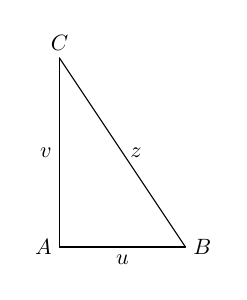
\begin{tikzpicture}[scale=0.8, transform shape,line cap=round,line join=round,>=latex,x=1.0cm,y=1.0cm]
\draw (0,0)--(2,0) node [midway, below] {$u$};
\draw (0,0)--(0,3) node [midway, left] {$v$};
\draw (2,0)--(0,3) node [midway, right] {$z$};
\node [left] at (0,0) {$A$};
\node [right] at (2,0) {$B$};
\node [above] at (0,3) {$C$};
\end{tikzpicture}
\par\end{center}

\end{example}

\end{onlyenv}



\begin{onlyenv}<2>

\begin{enumerate}
\item In these questions, you will always find several rates $u'$, $v'$
etc. given to you and one unknown rate $F'$.
\item Find out of what quantities these rates are, i.e., $u$ and $v$ etc.
\item Relate $F$ and $u$, $v$ by a function.
\item Differentiate this function with respect to time $t$ or whatever
the fundamental variable is. Then you get a relation between $F'$
and $u'$, $v'$ etc.
\end{enumerate}
\end{onlyenv}



\begin{onlyenv}<3>

\begin{example}
The diameter and height of a paper cup in the shape of a cone are
both $4$ inches, and water is leaking out at the rate of $\frac{1}{2}$
cubic inch per second. Find the rate of which the water level is dropping
when the diameter of the surface is $2$ inches.
\end{example}

\end{onlyenv}

\end{frame}




%\section[IndefInt]{Indefinite Integral}
\begin{frame}{Antiderivative/indefinite integral}


\[
\int f\left(x\right)\,\mathrm{d}x
\]



\pause{}
\begin{itemize}
\item antiderivative/indefinite integral of $f\left(x\right)$ is the function
whose derivative is $f\left(x\right)$.
\item For each function $f\left(x\right)$, its antiderivative is not unique.
\alert{Always remember to add $C$}.
\end{itemize}
\end{frame}

\begin{frame}{Basic formulas}


Remember all the formulas on p217 except for 13, 14, 17, 18, 19
\begin{example}
\[
\int\left(x^{4}+\sqrt[3]{x^{2}}-\frac{2}{x^{2}}-\frac{1}{3\sqrt[3]{x}}\right)\,\mathrm{d}x
\]

\end{example}

\end{frame}

\begin{frame}{Substitution rule}

\begin{onlyenv}<1>


If you have an integral of the form
\[
\int F\left(f\left(x\right)\right)f'\left(x\right)\,\mathrm{d}x
\]
then it equals
\[
\int F\left(u\right)\,\mathrm{d}u
\]
where $u=f\left(x\right)$.


Or you can consider that whenever a function passes through the differentiation
sign $\mathrm{d}$ from left to right, it becomes its antiderivative,
and when it passes from right to left, it becomes its derivative.
And everything after $\mathrm{d}$ can be viewed as a whole part.

\end{onlyenv}



\begin{onlyenv}<2>

\begin{example}
{\footnotesize{}
\[
\int\left(1-x^{2}\right)x\,\mathrm{d}x
\]
}{\footnotesize \par}
\end{example}


\pause{}
\begin{sol}
{\tiny{}
\begin{eqnarray*}
\int\left(1-x^{2}\right)x\,\mathrm{d}x & = & -\frac{1}{2}\int\left(1-x^{2}\right)\left(-2x\right)\,\mathrm{d}x\quad\boxed{u=1-x^{2}\,,u'=-2x}\\
 & = & -\frac{1}{2}\int u\cdot u'\,\mathrm{d}x\\
 & = & -\frac{1}{2}\int u\,\mathrm{d}u\\
 & = & -\frac{1}{2}\cdot\frac{1}{2}u^{2}\\
 & = & -\frac{1}{4}\left(1-x^{2}\right)^{2}\,.
\end{eqnarray*}
}{\tiny \par}
\end{sol}
\end{onlyenv}



\begin{onlyenv}<3>

\begin{example}
\[
\int\left(2x^{3}-1\right)^{5}x^{2}\,\mathrm{d}x\,,\int\sqrt[3]{1-x}\,\mathrm{d}x\,,\int\frac{e^{x}}{1-2e^{x}}\,\mathrm{d}x
\]
\[
\int\sin\left(1-2y\right)\,\mathrm{d}y\,,\int e^{\tan y}\sec^{2}y\,\mathrm{d}y\,,\int\frac{\cos\sqrt{x}}{\sqrt{x}}\,\mathrm{d}x
\]

\end{example}

\end{onlyenv}

\end{frame}

\begin{frame}{Integration by partial fractions}

\begin{onlyenv}<1>

\begin{enumerate}
\item Polynomial division;
\item Denominator factorization;
\item Determine coefficients;
\item Use \alert{substitution} and rule for $\frac{1}{x}$ to integrate.
\end{enumerate}
\end{onlyenv}



\begin{onlyenv}<2>

\begin{example}
\[
\int\frac{x^{2}-x+4}{x^{3}-3x^{2}+2x}\,\mathrm{d}x
\]

\end{example}

\end{onlyenv}

\end{frame}

\begin{frame}{Integration by parts}


\begin{eqnarray*}
\int f\left(x\right)g'\left(x\right)\,\mathrm{d}x & = & \int f\left(x\right)\,\mathrm{d}g\left(x\right)\\
 & = & f\left(x\right)g\left(x\right)-\int g\left(x\right)\,\mathrm{d}f\left(x\right)\\
 & = & f\left(x\right)g\left(x\right)-\int g\left(x\right)f'\left(x\right)\,\mathrm{d}x\,.
\end{eqnarray*}



\pause{}
\begin{example}
\[
\int x\cos x\,\mathrm{d}x\,,\int e^{x}\cos x\,,\int x^{4}\ln x\,\mathrm{d}x
\]

\end{example}


\pause{}


What can you conclude?

\end{frame}

\begin{frame}{Application of indefinite integral}

\begin{onlyenv}<1-2>

\begin{example}
The velocity of a particle moving along a line is given by $v\left(t\right)=4t^{3}-3t^{2}$
at time $t$. If the particle is initially at $x=3$ on the line,
find its position when $t=2$.
\end{example}


\pause{}
\begin{sol}
\[
s\left(t\right)=\int v\left(t\right)\,\mathrm{d}t
\]
\[
s\left(0\right)=3
\]

\end{sol}
\end{onlyenv}



\begin{onlyenv}<3>

\begin{example}
Suppose that $a\left(t\right)$, the acceleration of a particle at
time $t$, is given by $a\left(t\right)=4t-3$, that $v\left(1\right)=6$,
and that $f\left(2\right)=5$, where $f\left(t\right)$ is the position
function.
\begin{enumerate}
\item Find $v\left(t\right)$ and $f\left(t\right)$;
\item Find the position of the particle when $t=1$.
\end{enumerate}

\end{example}

\end{onlyenv}

\end{frame}




%\section[DefInt]{Definite Integrals}
\begin{frame}{Properties of definite integrals}

\begin{itemize}
\item 
\[
\int_{a}^{c}f\left(x\right)\,\mathrm{d}x+\int_{c}^{b}f\left(x\right)\,\mathrm{d}x=\int_{a}^{b}f\left(x\right)\,\mathrm{d}x
\]

\end{itemize}

\pause{}
\begin{itemize}
\item 
\[
\int_{a}^{b}f\left(x\right)\,\mathrm{d}x=-\int_{b}^{a}f\left(x\right)\,\mathrm{d}x
\]

\end{itemize}

\pause{}
\begin{itemize}
\item If $f\left(x\right)\le g\left(x\right)$ for all $x\in\left[a,b\right]$,
then
\[
\int_{a}^{b}f\left(x\right)\,\mathrm{d}x\le\int_{a}^{b}g\left(x\right)\,\mathrm{d}x\,.
\]

\end{itemize}
\end{frame}

\begin{frame}{Fundamental theorem of calculus}


\[
\int_{a}^{b}f\left(x\right)\,\mathrm{d}x=F\left(b\right)-F\left(a\right)
\]
where $F$ is the antiderivative of $f$. Or
\[
\frac{\mathrm{d}}{\mathrm{d}x}\int_{a}^{x}f\left(t\right)\,\mathrm{d}t=f\left(x\right)\,.
\]



\pause{}


Verbally, FTC says that integration and differentiation are two reverse
processes for a function.

\end{frame}

\begin{frame}{Evaluate definite integrals}

\begin{onlyenv}<1-2>

\begin{example}
\[
\int_{-1}^{2}\left(3x^{2}-2x\right)\,\mathrm{d}x
\]
\end{example}

\begin{uncoverenv}<2>

\begin{sol}
\begin{eqnarray*}
\int_{-1}^{2}\left(3x^{2}-2x\right)\,\mathrm{d}x & = & \left(x^{3}-x^{2}\right)\big|_{-1}^{2}\\
 & = & 6\,.
\end{eqnarray*}

\end{sol}
\end{uncoverenv}

\end{onlyenv}



\begin{onlyenv}<3-5>

\begin{example}
\[
\int_{5}^{8}\frac{\mathrm{d}y}{\sqrt{9-y}}
\]
\end{example}

\begin{onlyenv}<4>

\begin{sol}
{\scriptsize{}
\begin{eqnarray*}
\int_{5}^{8}\frac{\mathrm{d}y}{\sqrt{9-y}} & = & -\int_{5}^{8}\left(9-y\right)^{-\frac{1}{2}}\left(-1\right)\,\mathrm{d}y\\
 & = & -\int_{5}^{8}\left(9-y\right)^{-\frac{1}{2}}\,\mathrm{d}\left(9-y\right)\\
 & = & -2\left(9-y\right)^{\frac{1}{2}}\bigg|_{5}^{8}\\
 & = & 2
\end{eqnarray*}
}{\scriptsize \par}
\end{sol}
\end{onlyenv}



\begin{onlyenv}<5>

\begin{sol}
{\scriptsize{}
\begin{eqnarray*}
\int_{5}^{8}\frac{\mathrm{d}y}{\sqrt{9-y}} & = & -\int_{5}^{8}\left(9-y\right)^{-\frac{1}{2}}\left(-1\right)\,\mathrm{d}y\\
 & = & -\int_{5}^{8}\left(9-y\right)^{-\frac{1}{2}}\,\mathrm{d}\left(9-y\right)\\
 & = & -\int_{9-5}^{9-8}u^{-\frac{1}{2}}\,\mathrm{d}u\\
 & = & -2u^{\frac{1}{2}}\bigg|_{4}^{1}
\end{eqnarray*}
}{\scriptsize \par}
\end{sol}
\end{onlyenv}

\end{onlyenv}



\begin{onlyenv}<6-7>

\begin{example}
\[
\int_{0}^{1}e^{x}x\,\mathrm{d}x
\]
\end{example}

\begin{uncoverenv}<7>

\begin{sol}
{\scriptsize{}
\begin{eqnarray*}
\int_{0}^{1}e^{x}x\,\mathrm{d}x & = & \int_{0}^{1}x\,\mathrm{d}e^{x}\\
 & = & xe^{x}\bigg|_{0}^{1}-\int_{0}^{1}e^{x}\,\mathrm{d}x\\
 & = & e-0-\left(e-1\right)\\
 & = & 1
\end{eqnarray*}
}{\scriptsize \par}
\end{sol}
\end{uncoverenv}

\end{onlyenv}

\end{frame}

\begin{frame}{Represent functions using definite integral}

\begin{example}
\[
\frac{\mathrm{d}}{\mathrm{d}x}\int_{-1}^{x}\sqrt{1+\sin^{2}t}\,\mathrm{d}t\,,\frac{\mathrm{d}}{\mathrm{d}x}\int_{x}^{1}e^{-t^{2}}\,\mathrm{d}t
\]
\[
\frac{\mathrm{d}}{\mathrm{d}x}\int_{1}^{x}\frac{\mathrm{d}t}{3+t}
\]

\end{example}



\begin{example}
Find 
\[
\lim_{h\to0}\frac{1}{h}\int_{x}^{x+h}\sqrt{e^{t}-1}\,\mathrm{d}t\,.
\]

\end{example}

\end{frame}

\begin{frame}{Integrals involving parametrically defined functions}

\begin{example}
Evaluate $\int_{-2}^{2}y\,\mathrm{d}x$, where $x=2\sin\theta$, $y=3\cos\theta$.
\end{example}


\pause{}
\begin{example}
Sketch the curve given by $x=t-\sin t$, $y=1-\cos t$. Find out the
area between the curve and $x$-axis for one period.
\end{example}

\end{frame}

\begin{frame}{Riemann sum and approximation}

\begin{onlyenv}<1>


\[
\lim_{n\to\infty}\sum_{k=1}^{n}f\left(x_{k}\right)\Delta x_{k}=\int_{a}^{b}f\left(x\right)\,\mathrm{d}x\,.
\]
\[
\sum_{k=1}^{n}f\left(x_{k}\right)\Delta x_{k}\approx\int_{a}^{b}f\left(x\right)\,\mathrm{d}x\,.
\]


\end{onlyenv}



\begin{onlyenv}<2>

\begin{example}
Approximate $\int_{0}^{2}x^{3}\,\mathrm{d}x$ by using four subintervals
of equal width and calculating:
\begin{enumerate}
\item the left sum,
\item the right sum,
\item the midpoint sum,
\item the trapezoidal sum,
\item the integral.
\end{enumerate}

\end{example}

\end{onlyenv}

\end{frame}

\begin{frame}{Average value of a function}
The average value of a \alert{continuous} function equals the value
of the function at some point $c$ within the interval $(a,b)$.

\visible<2>{By FTC:}
\[
\frac{1}{b-a}\int_{a}^{b}f\left(x\right)\,\mathrm{d}x
\visible<2>{=\frac{F(b)-F(a)}{b-a}\,.}
\]
\visible<2>{\alert{How to interpret this?}}
\pause
\begin{example}
Find the average value of $y=1/x x$ on the interval $[1,4]$.
\end{example}
\pause
\begin{example}
Find the average rate of change of $y=\ln x$ on the interval $[1,4]$.
\end{example}

\end{frame}

\begin{frame}{More exercises}

\begin{example}
p409-27, 28; p410-53, 54, 56.
\end{example}

\begin{example}
p411-63, what is the average rate of change?
\end{example}

\end{frame}




%\section[AppofInt1]{Application of Integration in Geometry}
\begin{frame}{Area}


\[
y=f\left(x\right)\,,A=\int_{a}^{b}f\left(x\right)\,\mathrm{d}x\,.
\]



\[
\begin{cases}
x=f\left(t\right)\\
y=g\left(t\right)
\end{cases}\,,A=\int_{t_{1}}^{t_{2}}y\,\mathrm{d}x\,.
\]
\[
r=r\left(\theta\right)\,,A=\int_{\alpha}^{\beta}\frac{1}{2}r^{2}\,\mathrm{d}\theta\,.
\]
Always carefully justify the integral limits!
\begin{example}
p419-4, 6, 25
\end{example}

\end{frame}

\begin{frame}{Volume}

\begin{example}
p429-9
\end{example}

\begin{example}
p437-33
\end{example}

\begin{example}
The region bounded by $y=3x-x^{2}$ and $y=x$ is rotated about the
$y$-axis. Find the volume of the solid obtained.
\end{example}

\end{frame}

\begin{frame}{Arc length}


\[
y=f\left(x\right)\,,s=\int_{a}^{b}\sqrt{1+\left(\frac{\mathrm{d}y}{\mathrm{d}x}\right)^{2}}\,\mathrm{d}x\,;
\]
\[
\begin{cases}
x=x\left(t\right)\\
y=y\left(t\right)
\end{cases}\,,s=\int_{t_{1}}^{t_{2}}\sqrt{\left(\frac{\mathrm{d}x}{\mathrm{d}t}\right)^{2}+\left(\frac{\mathrm{d}y}{\mathrm{d}t}\right)^{2}}\,\mathrm{d}t\,;
\]
\[
r=r\left(\theta\right)\,,s=\int_{\alpha}^{\beta}\sqrt{r^{2}+\left(\frac{\mathrm{d}r}{\mathrm{d}\theta}\right)^{2}}\,\mathrm{d}\theta\,.
\]

\begin{example}
p441-3; p727-25, 26; p704-67.
\end{example}

\end{frame}

\begin{frame}{Improper integrals}

\begin{example}
\[
\int_{0}^{\infty}\frac{\mathrm{d}x}{\sqrt[3]{x+1}}\,,\int_{1}^{2}\frac{\mathrm{d}x}{\left(x-1\right)^{2}}\,.
\]

\end{example}

\begin{example}
(comparison test) Show that
\[
\int_{0}^{\infty}\frac{\mathrm{d}x}{\sqrt{x+x^{4}}}
\]
converges.
\end{example}



\begin{example}
p555-55
\end{example}

\end{frame}




%\section[AppofInt2]{Further Applications of Integration}
\begin{frame}{Motion}

\begin{onlyenv}<1>

\begin{itemize}
\item Integration of velocity is displacement;
\item Integration of acceleration is the variation of velocity;
\item Integration of speed is distance.\end{itemize}
\begin{example}
If a body moves along a straight line with velocity $v=t^{3}-3t^{2}$,
find the distance traveled between $t=1$ and $t=4$.
\end{example}

\end{onlyenv}



\begin{onlyenv}<2>

\begin{example}
A praticle $P$ moves along a curve so that its acceleration is given
by
\[
\mathbf{a}=\left(-4\cos2t,-2\sin t\right)\,,-\frac{\pi}{2}\le t\le\frac{\pi}{2}\,;
\]
when $t=0$, the particle is at $\left(1,0\right)$ with $\frac{\mathrm{d}x}{\mathrm{d}t}=0$,
and $\frac{\mathrm{d}y}{\mathrm{d}t}=2$.
\begin{enumerate}
\item Find the position vector $\mathbf{R}$ at any time $t$.
\item Find a integral representing the distance $P$ travels from $t=0$
to $t=2$.
\end{enumerate}

\end{example}

\end{onlyenv}



\begin{onlyenv}<3>

\begin{example}
(net change) After $t$ minutes, a chemical is decomposing at the
rate of $10e^{-t}$ grams per minute. Find the amount that has decomposed
during the first $3$ minutes.
\end{example}



\begin{example}
Suppose a rumor is spreading at the rate of $f\left(t\right)=100e^{-0.2t}$
new people per day. Find the number of people who hear the rumor during
the $5$th and $6$th days.
\end{example}

\end{onlyenv}

\end{frame}




%\section[DiffEqn]{Differential Equations}
\begin{frame}{Slope field}

\begin{example}
p395-22, 23
\end{example}



\begin{example}
The stock price is modeled by the following differential equation
\[
\frac{\mathrm{d}P}{\mathrm{d}t}=-P^{2}+2P+\sqrt{P}
\]
At which price level the price increase fastest?
\end{example}

\end{frame}

\begin{frame}{Solving equations}

\begin{example}
(separate equations) p394-13, 14.
\end{example}

\end{frame}

\begin{frame}{Exponential model}

\begin{example}
The bacteria in a certain culture increase continuously at a rate
proportional to the number present. If the number triples in $6$
hours, how many will there be in $15$ hours?
\end{example}



\begin{example}
Radium-226 decays at a rate proportional to the quantity present.
Its half-life is 1612 years. How long will it take for one quarter
of a given quantity of radium-226 to decay?
\end{example}

\end{frame}

\begin{frame}{Newton's law of cooling}

\begin{example}
A hot object cools at a rate proportional to the difference between
its own temperature and that of its environment. If roast at room
temperature $68^{\circ}\mathrm{F}$ is put into a $20^{\circ}\mathrm{F}$
freezer, and if, after $2$ hours, the temperature of the roast is
$40^{\circ}\mathrm{F}$:
\begin{enumerate}
\item What is its temperature after $5$ hours?
\item How long will it take for the temperature of the roast to fall to
$21^{\circ}\mathrm{F}$?
\end{enumerate}

\end{example}

\end{frame}

\begin{frame}{Logistic growth}

\begin{example}
Because of limited food and space, a squirrel population cannot exceed
\alert<2>{$1000$}. When there were $100$ squirrels $2$ years ago,
the \alert<2>{increase rate} of the population is $10$ squirrels
per year.
\begin{enumerate}
\item Find the \alert<2>{relative growth rate} of this population and write
down the differential equation.
\item Sketch the solution curve of the initial condition given above.
\item Use \alert<2>{Euler's method} to estimate the population now by 2
steps.
\end{enumerate}

\end{example}

\end{frame}




\section{Sequences and Series}
\begin{frame}{Sequences and series}
    \[
    \lim_{n\to\infty}\frac{1}{n}\quad\sum_{n=1}^{\infty}\frac{1}{n}
    \]
    \pause{}

    \[
    \lim_{n\to\infty}\frac{1}{2^{n}}\quad\sum_{n=1}^{\infty}\frac{1}{2^{n}}
    \]
    \pause{}
    
    \[
    \lim_{n\to\infty}\frac{3n^{4}+5}{4n^{4}-7n^{2}+9}
    \]
\end{frame}

\begin{frame}{Convergence of series}
    The definition of sum of infinite many terms:
    \[
    \sum_{n=1}^{\infty}a_{n}=\lim_{N\to\infty}\sum_{n=1}^{N}a_{n}\,.
    \]
    When the limit exists, it is called convergent.
    
    
    For a series to be convergent, its ``tail'' must shrink very quickly
    \[
    \lim_{n\to\infty}a_{n}=0\,.
    \]
    When $\sum\left|a_{n}\right|$ is convergent, we call the series $\sum a_{n}$
    \alert{absolutely convergent}. What is \alert{conditional convergence}?

\end{frame}

\begin{frame}{Geometric series}


\begin{eqnarray*}
\sum_{n=1}^{\infty}ar^{n-1} & = & \lim_{N\to\infty}\frac{a\left(1-r^{N}\right)}{1-r}\\
 & = & \frac{a}{1-r}\,,
\end{eqnarray*}
when \uncover<2>{$\left|r\right|<1$.}

\pause{}


So no matter $r$ is postive or negative, if a geometric series converges,
it converges absolutely.

\end{frame}

\begin{frame}{$p$-series}


\[
\sum_{n=1}^{\infty}\frac{1}{n^{p}}
\]

\begin{itemize}
\item It is convergent when $p>1$;
\item It is divergent when $p\le1$.
\item $\sum_{n=1}^{\infty}\frac{\left(-1\right)^{n}}{n^{p}}$ is always
convergent, but not always absolutely. Why?
\end{itemize}
\end{frame}

\begin{frame}{Telescopic series}


\begin{eqnarray*}
\sum_{n=1}^{\infty}\frac{1}{n\left(n+1\right)} & = & \lim_{N\to\infty}\sum_{n=1}^{N}\left(\frac{1}{n}-\frac{1}{n+1}\right)\\
 & = & \lim_{N\to\infty}\left(1-\frac{1}{N+1}\right)\\
 & = & 1\,.
\end{eqnarray*}

\begin{example}
\[
\sum_{n=1}^{\infty}\frac{1}{n\left(n+2\right)}
\]

\end{example}

\end{frame}

\begin{frame}{Tests for convergence}

\begin{onlyenv}<1>

\begin{itemize}
\item Ratio test.
\[
\lim_{n\to\infty}\left|\frac{a_{n+1}}{a_{n}}\right|=L
\]

\item Comparison test. Only for positive series. Want to show convergence,
amplify it; want to show divergence, shrink it.
\item Integral test. Only for positive series. The integral converges $\int_{1}^{\infty}f\left(n\right)\,\mathrm{d}n$
iff the series $\sum f\left(n\right)$ converges.
\item Alternating series test.
\[
\left|a_{n+1}\right|\le\left|a_{n}\right|\mbox{ and }\lim_{n\to\infty}a_{n}=0\,.
\]

\end{itemize}
\end{onlyenv}



\begin{onlyenv}<2>

\begin{example}
\[
\sum_{n=1}^{\infty}\frac{1}{1+n^{4}}\,,\sum_{n=1}^{\infty}\left(\frac{n}{2n+1}\right)^{n}\,,\sum_{n=1}^{\infty}\frac{\sin\frac{n\pi}{3}}{n^{2}}
\]

\end{example}



\begin{example}
\[
\sum_{n=1}^{\infty}\frac{\left(-1\right)^{n+1}}{\sqrt[3]{n+1}}
\]

\end{example}

\end{onlyenv}

\end{frame}

\begin{frame}{Power series}


\[
\sum_{k=0}^{\infty}c_{k}x^{k}\quad\sum_{k=0}^{\infty}c_{k}\left(x-a\right)^{k}
\]
Use ratio test to control radius of convergence.



\begin{example}
For what $x$ does
\[
\sum_{n=1}^{\infty}\frac{\left(-1\right)^{n-1}x^{n-1}}{n+1}
\]
converge?
\end{example}

\end{frame}

\begin{frame}{Taylor series}
Some (\alert{analytic}) functions can be expressed as power series for all real numbers
or within some interval.
\[
f\left(x\right)=\sum_{n=0}^{\infty}\frac{f^{\left(n\right)}\left(a\right)}{n!}\left(x-a\right)^{n}\,\mbox{for }\left|x-a\right|<R\,.
\]

\begin{example}
p667-50
\end{example}

\end{frame}

\begin{frame}{Counterexample}
        \only<1>{
        Note that it is true that with some regularity assumptions
        \[f(x)=\sum_{k=0}^{n}\frac{f^{(k)}(a)}{k!}\left(x-a\right)^k+\frac{f^{(k+1)}(\xi)}{(k+1)!}\left(x-a\right)^{(k+1)}\,.\]
        But it is not true that
        \[f(x)=\sum_{k=0}^{\infty}\frac{f^{(k)}(a)}{k!}\left(x-a\right)^k\,,\]
        even when the series converges in $(a-R,a+R)$ for some $R>0$.
}
        \only<2>{
        See the following example (by Cauchy)
        \[f(x)=
        \begin{cases}
                e^{-1/x^2} & x\ne 0\,;\\
                0 & x=0\,.
        \end{cases}\]
        The remainder formula is still correct but the derivatives oscillate severely.
}
\end{frame}

\begin{frame}{Basic series}


$\sin x$, $\cos x$, $e^{x}$, $\ln\left(1+x\right)$, $\frac{1}{1-x}$

\end{frame}

\begin{frame}{Calculus on series}

\begin{onlyenv}<1>
Within the interval of convergence, series can be added, multiplied
by a constant, integrated and differentiated \alert{term by term}.
For example,
\[
\arctan x=\int_{0}^{x}\frac{\mathrm{d}t}{1+t^{2}}=\sum_{n=0}^{\infty}\int\left(-1\right)^{n}t^{2n}\,\mathrm{d}t\,.
\]
\end{onlyenv}

\begin{onlyenv}<2>

\begin{example}
    p687-6(d), 10, 20
\end{example}

\end{onlyenv}

\end{frame}

\begin{frame}{Approximate functions}

\begin{onlyenv}<1>
\[
f\left(x\right)\approx\sum_{n=1}^{N}\frac{f^{\left(n\right)}\left(a\right)}{n!}\left(x-a\right)^{n}
\]
with the error
\[
\left|f\left(x\right)-\sum_{n=1}^{N}\frac{f^{\left(n\right)}\left(a\right)}{n!}\left(x-a\right)^{n}\right|\le\left|\frac{{\displaystyle \max_{\left|t-a\right|\le R}}f^{\left(n+1\right)}\left(t\right)}{\left(n+1\right)!}\left(x-a\right)^{n+1}\right|
\]
for $\left|x-a\right|\le R$.

If it is an alternating series with $\left|a_{n+1}\right|<\left|a_{n}\right|$,
then
\[
\left|f\left(x\right)-\sum_{n=1}^{N}\frac{f^{\left(n\right)}\left(a\right)}{n!}\left(x-a\right)^{n}\right|\le\left|\frac{f^{\left(n+1\right)}\left(a\right)}{\left(n+1\right)!}\left(x-a\right)^{n+1}\right|\,.
\]
\end{onlyenv}

\begin{onlyenv}<2>

\begin{example}
For what values of $x$ is the approximate formula
\[
\ln\left(1+x\right)\approx x-\frac{x^{2}}{2}
\]
accurate to $0.001$?\end{example}

\end{onlyenv}

\end{frame}





\end{document}
